% TODO move plots from appendix to text and elaborate on TC Genesis regions
\chapter{Additional TC Genesis Plots}\label{sec:genesis-appendix}

\begin{figure}[ht]
	\centering
	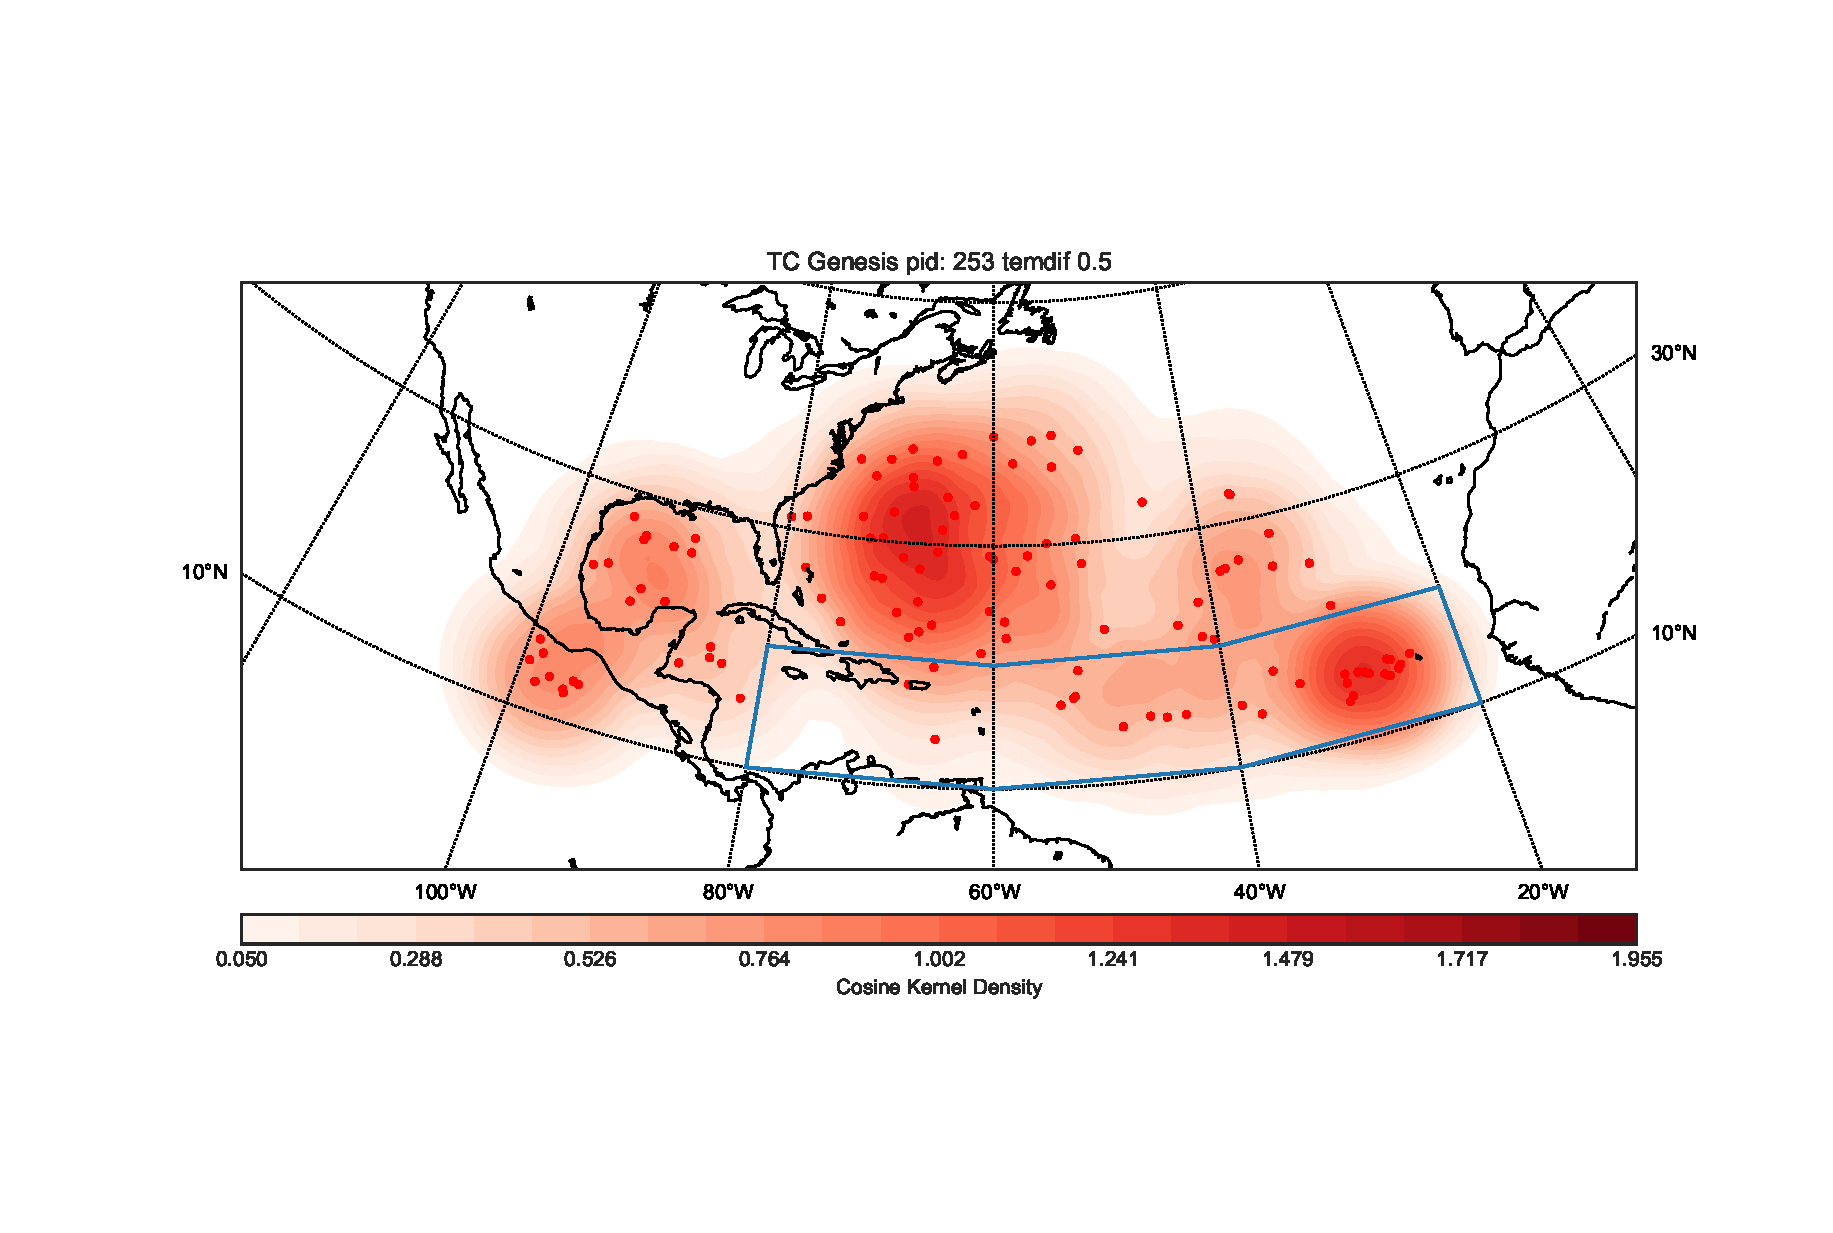
\includegraphics[width=0.7\textwidth]{img/genesis_plot_temdif05.eps}
	\caption{Genesis spots and density for temdif = 0.5.}
\end{figure}
\begin{figure}[ht]
	\centering
	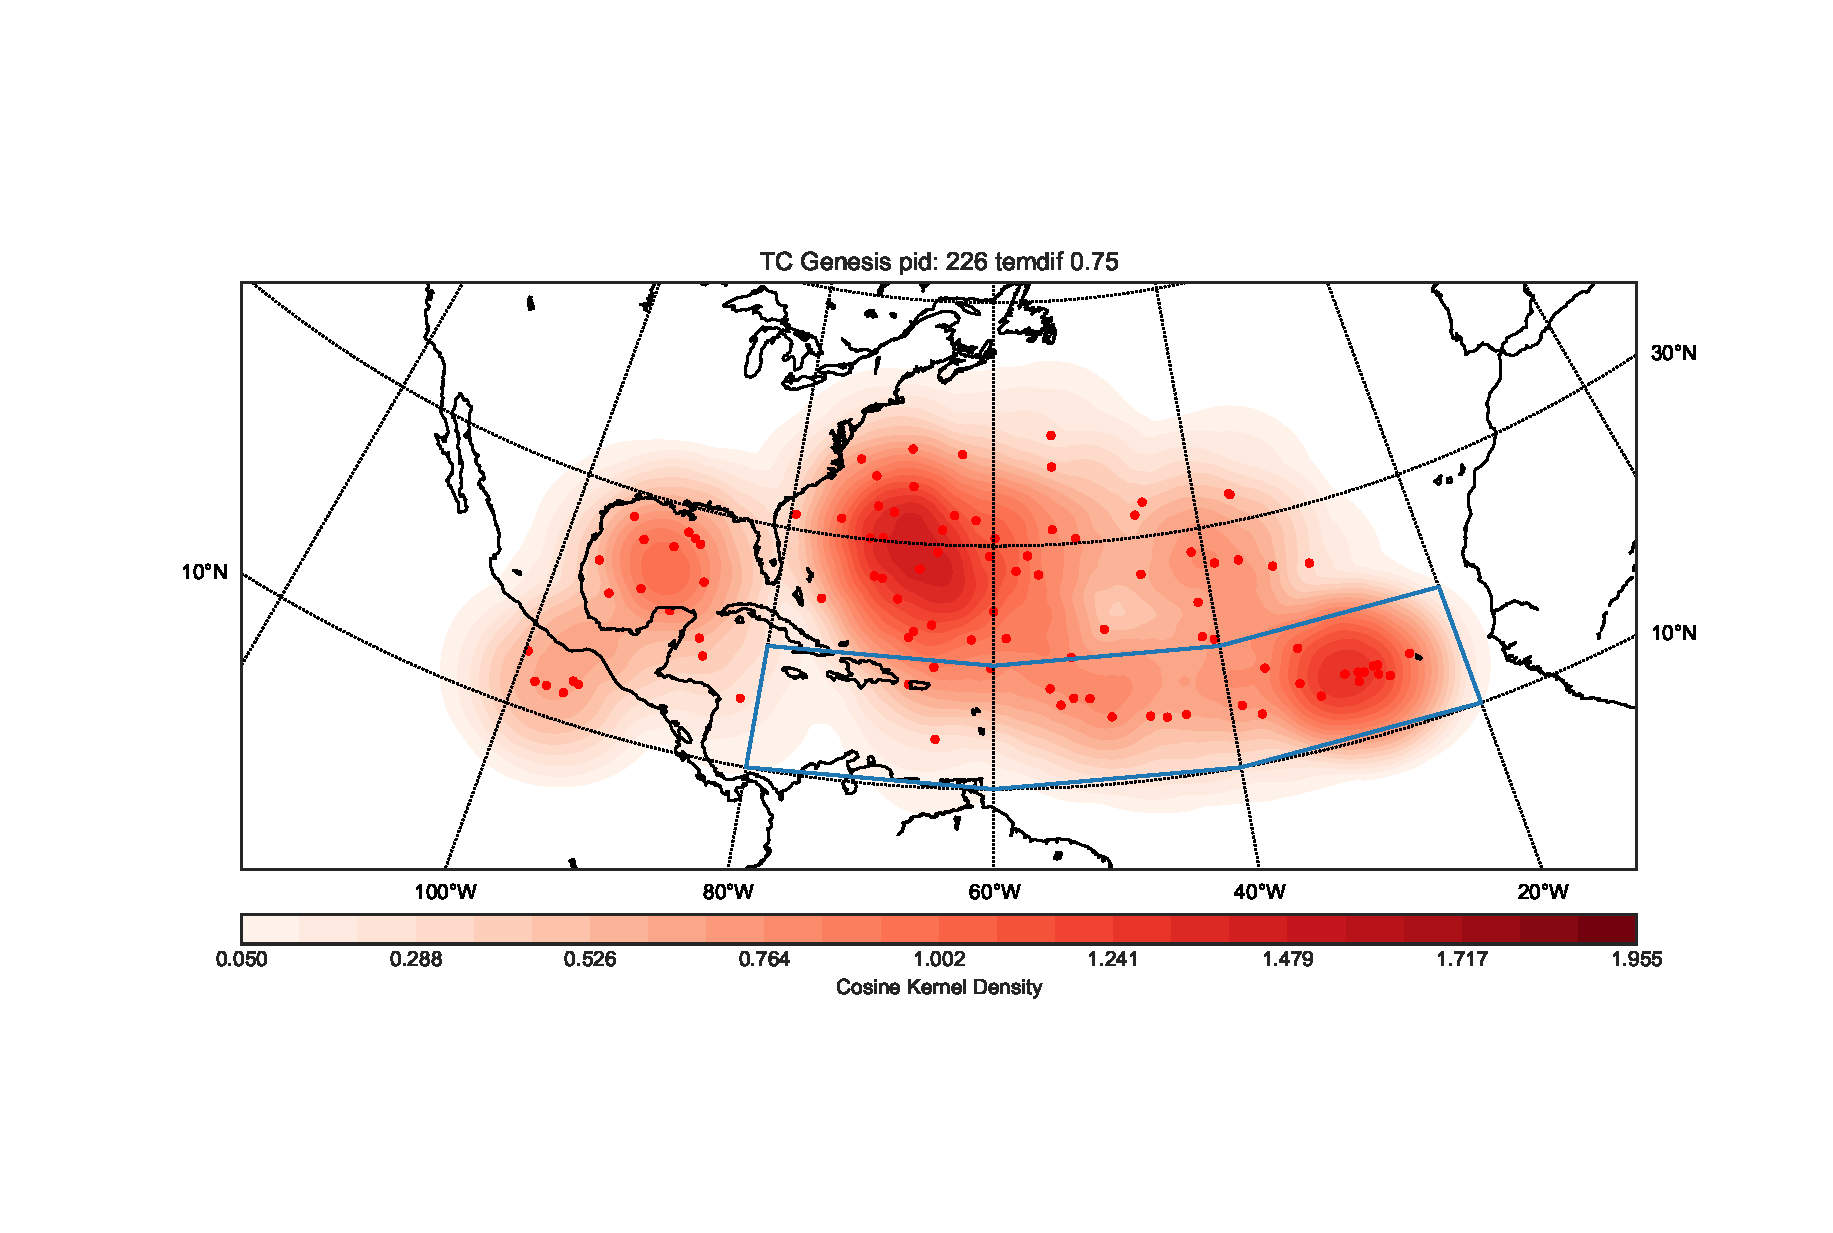
\includegraphics[width=0.7\textwidth]{img/genesis_plot_temdif075.eps}
	\caption{Genesis spots and density for temdif = 0.75.}
\end{figure}
\begin{figure}[ht]
	\centering
	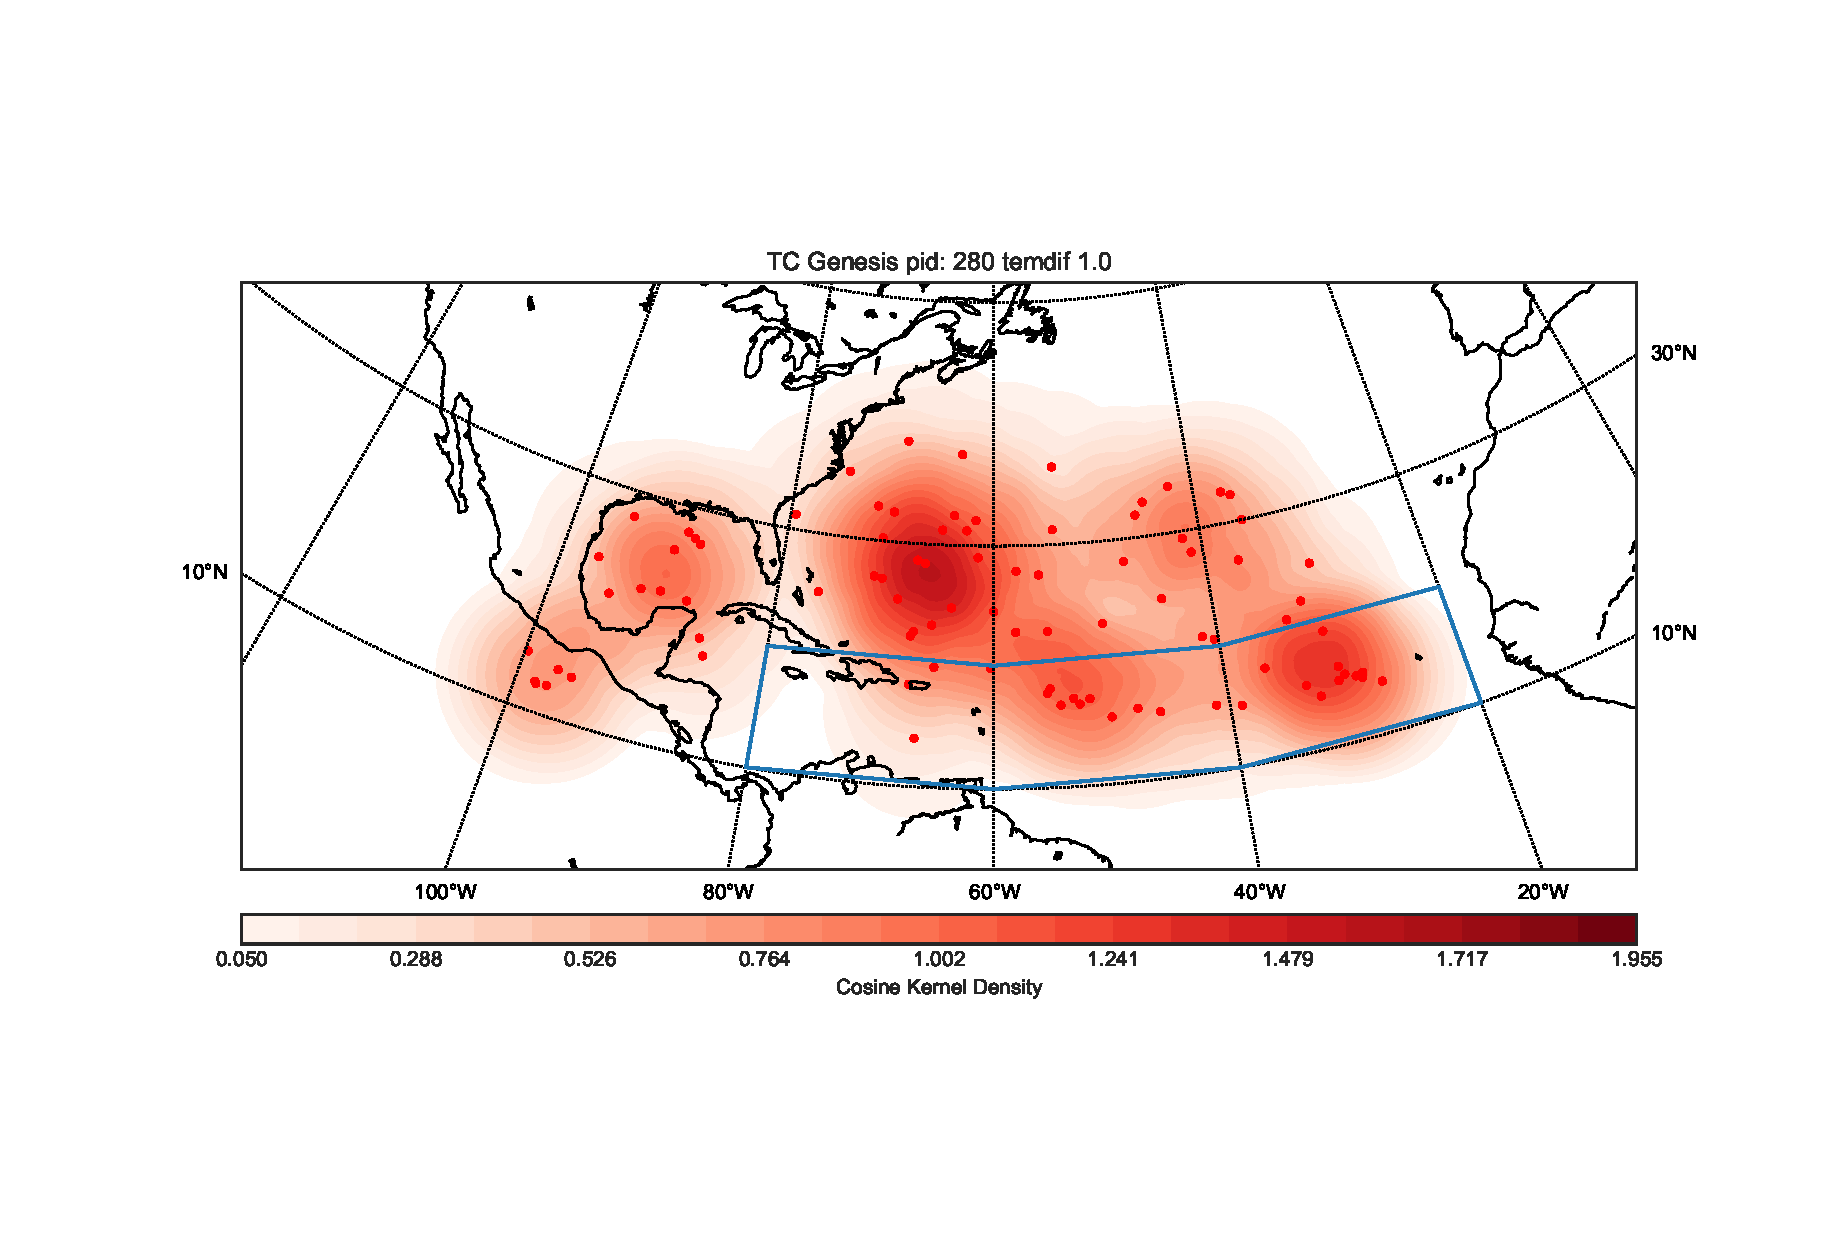
\includegraphics[width=0.7\textwidth]{img/genesis_plot_temdif1.eps}
	\caption{Genesis spots and density for temdif = 1.0.}
\end{figure}
\begin{figure}[ht]
	\centering
	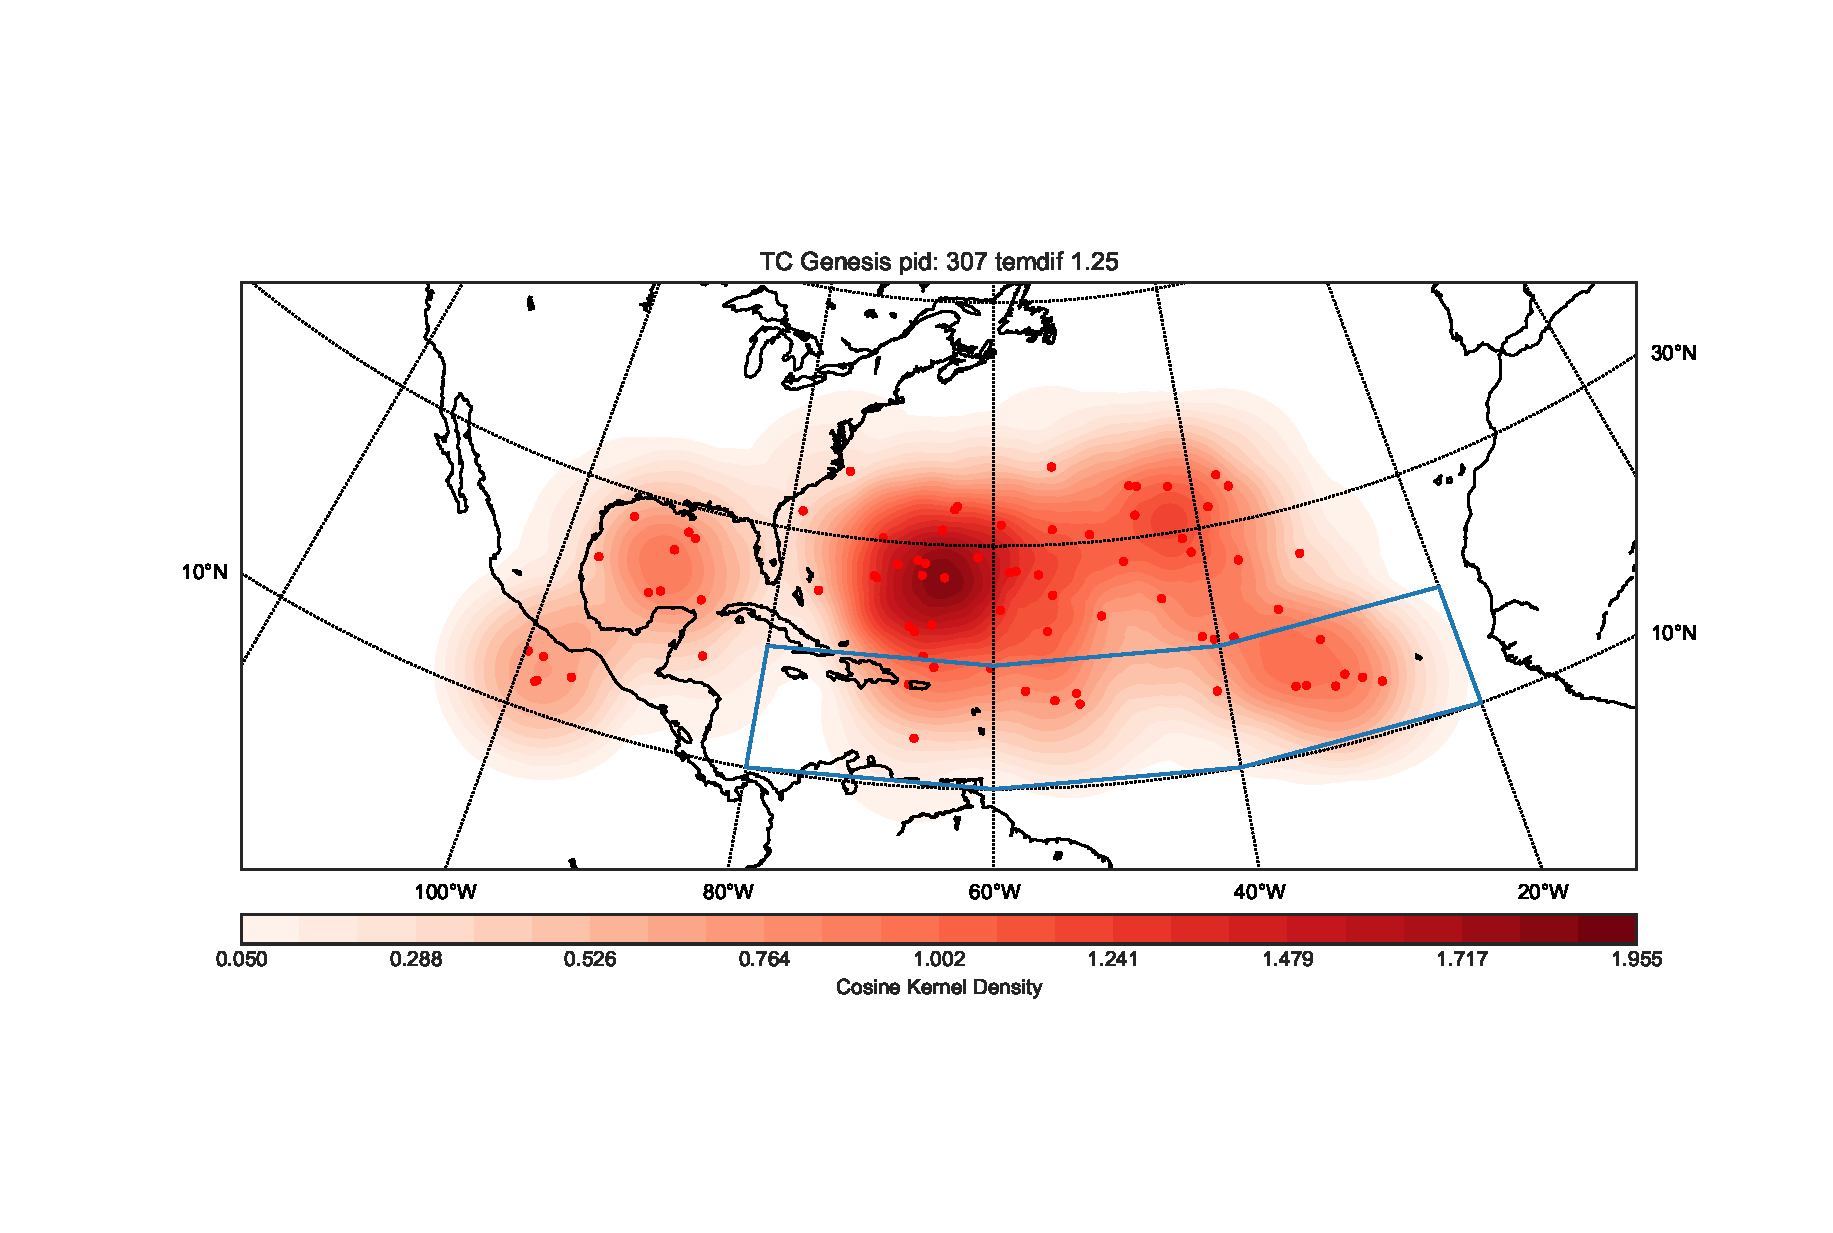
\includegraphics[width=0.7\textwidth]{img/genesis_plot_temdif125.eps}
	\caption{Genesis spots and density for temdif = 1.25.}
\end{figure}
\begin{figure}[ht]
	\centering
	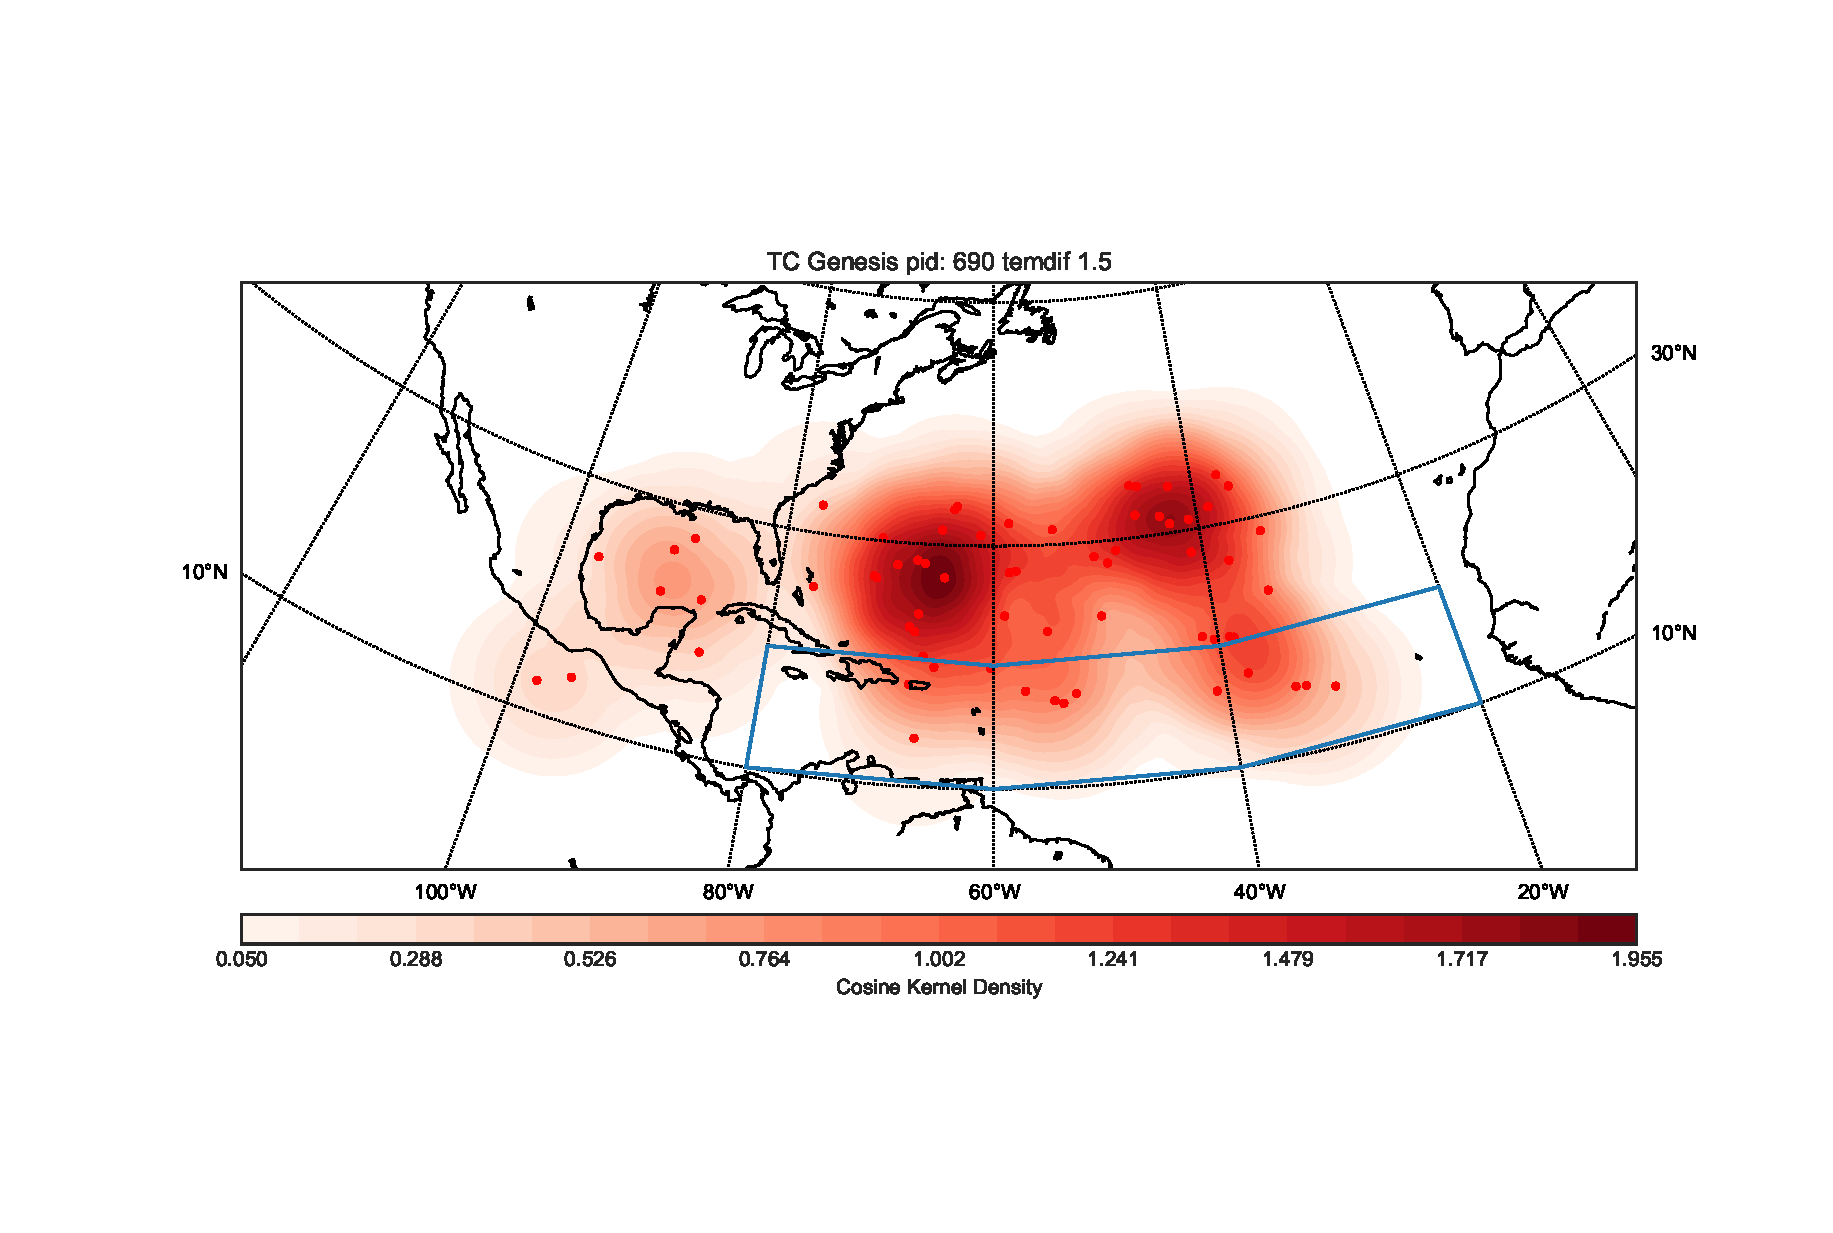
\includegraphics[width=0.7\textwidth]{img/genesis_plot_temdif15.eps}
	\caption{Genesis spots and density for temdif = 1.5.}
\end{figure}

\chapter{Lifetime dependence on the warm core criterion}\label{sec:lifetime-appendix}

\begin{figure}[ht]
	\centering
	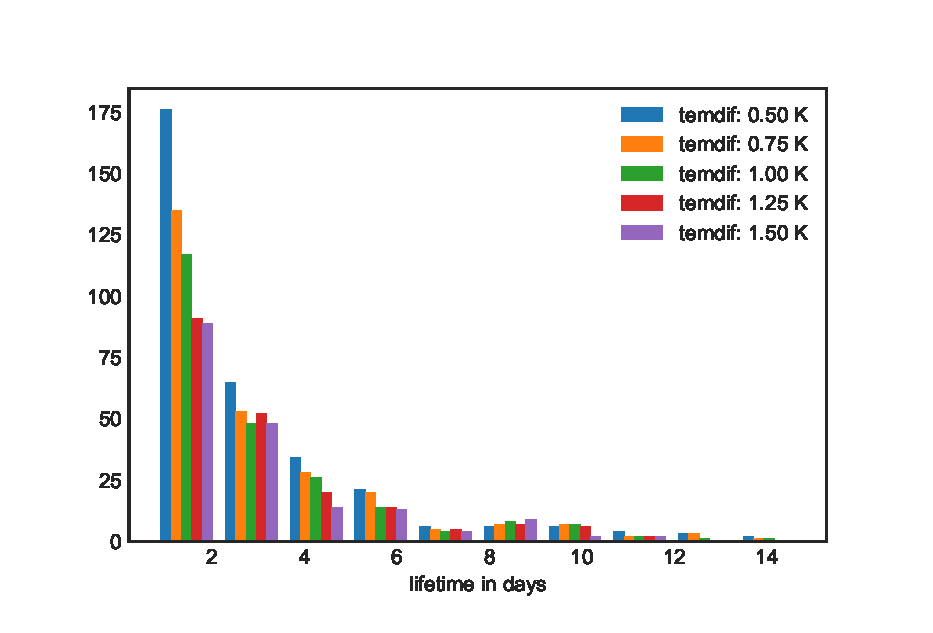
\includegraphics[width=0.7\textwidth]{img/lifetime_for_different_temdif.eps}
	\caption{Histogram showing the number of TCs with a certain lifetime in days.}
\end{figure}

 
 
%---------------------------------------------------------------------------
% Symbols

\chapter*{Nomenclature}\label{chap:symbole}
 \addcontentsline{toc}{chapter}{Nomenclature}
 
\section*{Acronyms and Abbreviations}
\begin{tabbing}
 \hspace*{1.6cm}  \= \kill
 ETH \> Eidgen\"{o}ssische Technische Hochschule \\[0.5ex]
 TC \> Tropical Cyclone \\[0.5ex]
 DWD \> German Weather Service\\[0.5ex]
 MPIM \> Max Planck Institute for Meteorology\\[0.5ex]
ICON \> Icosahedral Nonhydrostatic Model developed by the DWD and the
MPIM\\[0.5ex]
SST \> sea surface temperature\\[0.5ex]
SLP \> sea level pressure\\[0.5ex]
MDR \> main development region  \\[0.5ex]
\end{tabbing}

%---------------------------------------------------------------------------
